% ncse_new/\problems/ch_piecewisepolynomials/ex_CubicSplines.tex
%  solution:  ex_CubicSpline.m  ex_CubicSpline.eps

\begin{problem}[Zeros of orthogonal polynomials \coreproblem]
 This problem combines elementary methods for zero finding with 3-term recursions satisfied by orthogonal polynomials. 
  
The zeros of the Legendre polynomial $P_n$ (see \lref{def:Legendrepol}) are the $n$ Gauss points $\xi^n_j$, $j=1,\dots,n$. In this problem we compute the Gauss points by zero finding methods applied to $P_n$. The 3-term recursion \lref{eq:Legpol} for Legendre polynomials will play an essential role. Moreover, recall that, by definition, the Legendre polynomials are $L^2(]-1,1[)$-orthogonal.

% SUBPROBLEM 1
\begin{subproblem}[5]\label{subpb:inter}
Prove the following interleaving property of the zeros of the Legendre polynomials. For all $n\in\n_0$ we have
\begin{equation*}
-1<\xi^n_j<\xi^{n-1}_j<\xi^n_{j+1}<1,\qquad j=1,\dots,n-1.
\end{equation*}
 \begin{hint}
You may follow these steps:
\begin{enumerate}\itemsep0pt
\item Understand that it is enough to show that every pair of zeros $(\xi^n_l,\xi^n_{l+1})$ of $P_n$ is separated by a zero of $P_{n-1}$.
\item Argue by contradiction.
\item By considering the auxiliary polynomial $\prod_{j\neq l,l+1} (t-\xi_j^n)$ and the fact that the Gauss quadrature is exact on $\Pol{2n-1}$ prove that $P_{n-1}(\xi_l^n)=P_{n-1}(\xi_{l+1}^n)=0$.
\item Choose $s\in \Pol{n-2}$ such that $s(\xi^n_j)=P_{n-1}(\xi_j^n)$ for every $j\neq l,l+1$, and using again that  Gauss quadrature is exact on $\Pol{2n-1}$ obtain a contradiction.
\end{enumerate}
\end{hint}

\begin{solution}
By \lref{lem:gn}, $P_n$ has exactly $n$ distinct zeros in $]-1,1[$. Therefore, it is enough to prove that every pair of zeros of $P_n$ is separated by one zero of $P_{n-1}$. By contradiction, assume that there exists $l=1,\dots,n-1$ such that $]\xi^n_l,\xi_{l+1}^n[$ does not contain any zeros of $P_{n-1}$. As a consequence, $P_{n-1}(\xi^n_l)$ and $P_{n-1}(\xi^n_{l+1})$ have the same sign, namely
\begin{equation}\label{eq:separate}
P_{n-1}(\xi^n_l) P_{n-1}(\xi^n_{l+1})\ge 0.
\end{equation}

Recall that, by construction, we have the following orthogonality property
\begin{equation}\label{eq:orthog}
\int_{-1}^1P_{n-1}q\,dt=0,\qquad q\in\Pol{n-2}.
\end{equation}

Consider the auxiliary polynomial
\[
q(t)=\prod_{j\neq l,l+1} (t-\xi^n_j).
\]
By construction, $q\in\Pol{n-2}$, whence $P_{n-1}q\in\Pol{2n-3}$. Thus, using \eqref{eq:orthog} and the fact that Gaussian quadrature is exact on $P_{2n-1}$ we obtain
\[
0 = \int_{-1}^1P_{n-1}q\,dt 
 = \sum_{j=1}^n w_j P_{n-1}(\xi_j^n) q(\xi^n_j) 
 = w_l P_{n-1}(\xi_l^n) q(\xi^n_l) + w_{l+1} P_{n-1}(\xi_{l+1}^n) q(\xi^n_{l+1}).
\]
Hence
\[
\left[ w_l P_{n-1}(\xi_l^n) q(\xi^n_l) \right] \left[ w_{l+1} P_{n-1}(\xi_{l+1}^n) q(\xi^n_{l+1})\right]\le 0.
\]
On the other hand, by \lref{lem:gw} we have $w_l ,w_{l+1}>0$. Moreover, by construction of $q$ we have that $q(\xi^n_l)q(\xi^n_{l+1})>0$. Combining these properties with \eqref{eq:separate} we obtain that
\[
P_{n-1}(\xi_l^n)=P_{n-1}(\xi_{l+1}^n)=0.
\]

Choose now $s\in \Pol{n-2}$ such that $s(\xi^n_j)=P_{n-1}(\xi_j^n)$ for every $j\neq l,l+1$. Using again \eqref{eq:orthog} and the fact that Gaussian quadrature is exact on $P_{2n-1}$ we obtain
\[
0=\int_{-1}^1 P_{n-1} s\,dt=\sum_{j=1}^n w_j P_{n-1}(\xi_j^n) s(\xi_j^n)= \sum_{j\neq l,l+1} w_j (P_{n-1}(\xi_j^n))^2.
\]
Since $P_{n-1}$ has only $n-1$ zeros and the weights $w_j$ are all positive, the right hand side of this equality is strictly positive, thereby contradicting the equality itself.

\textbf{Solution 2: }
There is a shorter proof of this fact based on the recursion formula \lref{eq:Legpol}. We sketch the main steps.

We will prove the statement by induction. If $n=1$ there is nothing to prove. Suppose now that the statement is true for $n$. By \lref{eq:Legpol} we have $P_{n+1}(\xi^n_j)=-\frac{n}{n+1}P_{n-1}(\xi^n_j)$ for every $j=1,\dots,n$. Further, since the statement is true for $n$ we have $(-1)^{n-j}P_{n-1}(\xi^n_j)>0$. Therefore
\begin{equation}\label{eq:last}
(-1)^{n+1-j}P_{n+1}(\xi^n_j)>0,\qquad j=1,\dots,n.
\end{equation}
Since the leading coefficient of $P_{n+1}$ is positive, we have $P_{n+1}(x)>0$ for all $x>\xi^{n+1}_{n+1}$ and $(-1)^{n+1}P_{n+1}(x)>0$ for all $x<\xi^{n+1}_{1}$. Combining these two inequalities with \eqref{eq:last} yields the result for $n+1$.
\end{solution}
\end{subproblem}


% SUBPROBLEM 2
\begin{subproblem}[1]\label{subpb:2}
By differentiating \lref{eq:Legpol} derive a combined 3-term recursion for the sequences $(P_n)_n$ and $(P'_n)_n$.
\begin{solution}
Differentiating \lref{eq:Legpol} immediately gives
\begin{equation*}
P_{n+1}'(t)=\frac{2n+1}{n+1}P_n(t) + \frac{2n+1}{n+1} t P_n'(t)-\frac{n}{n+1}P'_{n-1}(t),\quad P_0'=0,\quad P_1'=1,
\end{equation*}
which combined with \lref{eq:Legpol} gives the desired recursions.
\end{solution}
\end{subproblem}

% SUBPROBLEM 3
\begin{subproblem}[2]
Use the recursions obtained in \ref{subpb:2} to write a C++ function
\begin{lstlisting}
void legvals(const Eigen::VectorXd &x, Eigen::MatrixXd &Lx, Eigen::MatrixXd &DLx)
\end{lstlisting}
that fills the matrices \texttt{Lx} and \texttt{DLx} in $\R^{N\times (n+1)}$ with the values $(P_k(x_j))_{jk}$ and $(P'_k(x_j))_{jk}$, $k=0,\dots,n$, $j=0,\dots,N-1$, for an input vector $x\in \R^N$ (passed in \texttt{x}).
\begin{solution}
See file \texttt{legendre.cpp}.
\end{solution}
\end{subproblem}

% SUBPROBLEM 4
\begin{subproblem}[3]
We can compute the zeros of $P_k$, $k=1,\dots,n$, by means of the secant rule (see \lref{par:secant}) using the endpoints $\{-1,1\}$ of the interval and the zeros of the previous Legendre polynomial as initial guesses, see \ref{subpb:inter}. We opt for a correction based termination criterion (see \lref{sec:termination-criteria-1}) based on prescribed relative and absolute tolerance (see \lref{mc:secant}).

Write a C++ function
\begin{lstlisting}
MatrixXd gaussPts(int n, double rtol=1e-10, double atol=1e-12)
\end{lstlisting}
that computes the Gauss points $\xi^k_j\in [-1,1]$, $j=1,\dots,k$, $k=1,\dots,n$, using the zero finding approach outlined above. The Gauss points should be returned in  an upper triangular $n\times n$-matrix.
\begin{hint}
For simplicity, you may want to write a C++ function
\begin{lstlisting}
double Pkx(double x, int k)
\end{lstlisting}
that computes $P_k(x)$ for a scalar $x$. Reuse parts of the function \texttt{legvals}.
\end{hint}
\begin{solution}
See file \texttt{legendre.cpp}.
\end{solution}
\end{subproblem}

% SUBPROBLEM 5
\begin{subproblem}[2]
Validate your implementation of the function \texttt{gaussPts} with $n=8$ by computing the values of the Legendre polynomials in the zeros obtained (use the function \texttt{legvals}). Explain the failure of the method.
\begin{hint}
See Figure~\ref{fig:secant}.
\begin{figure}[hbt]
\hspace{8mm}
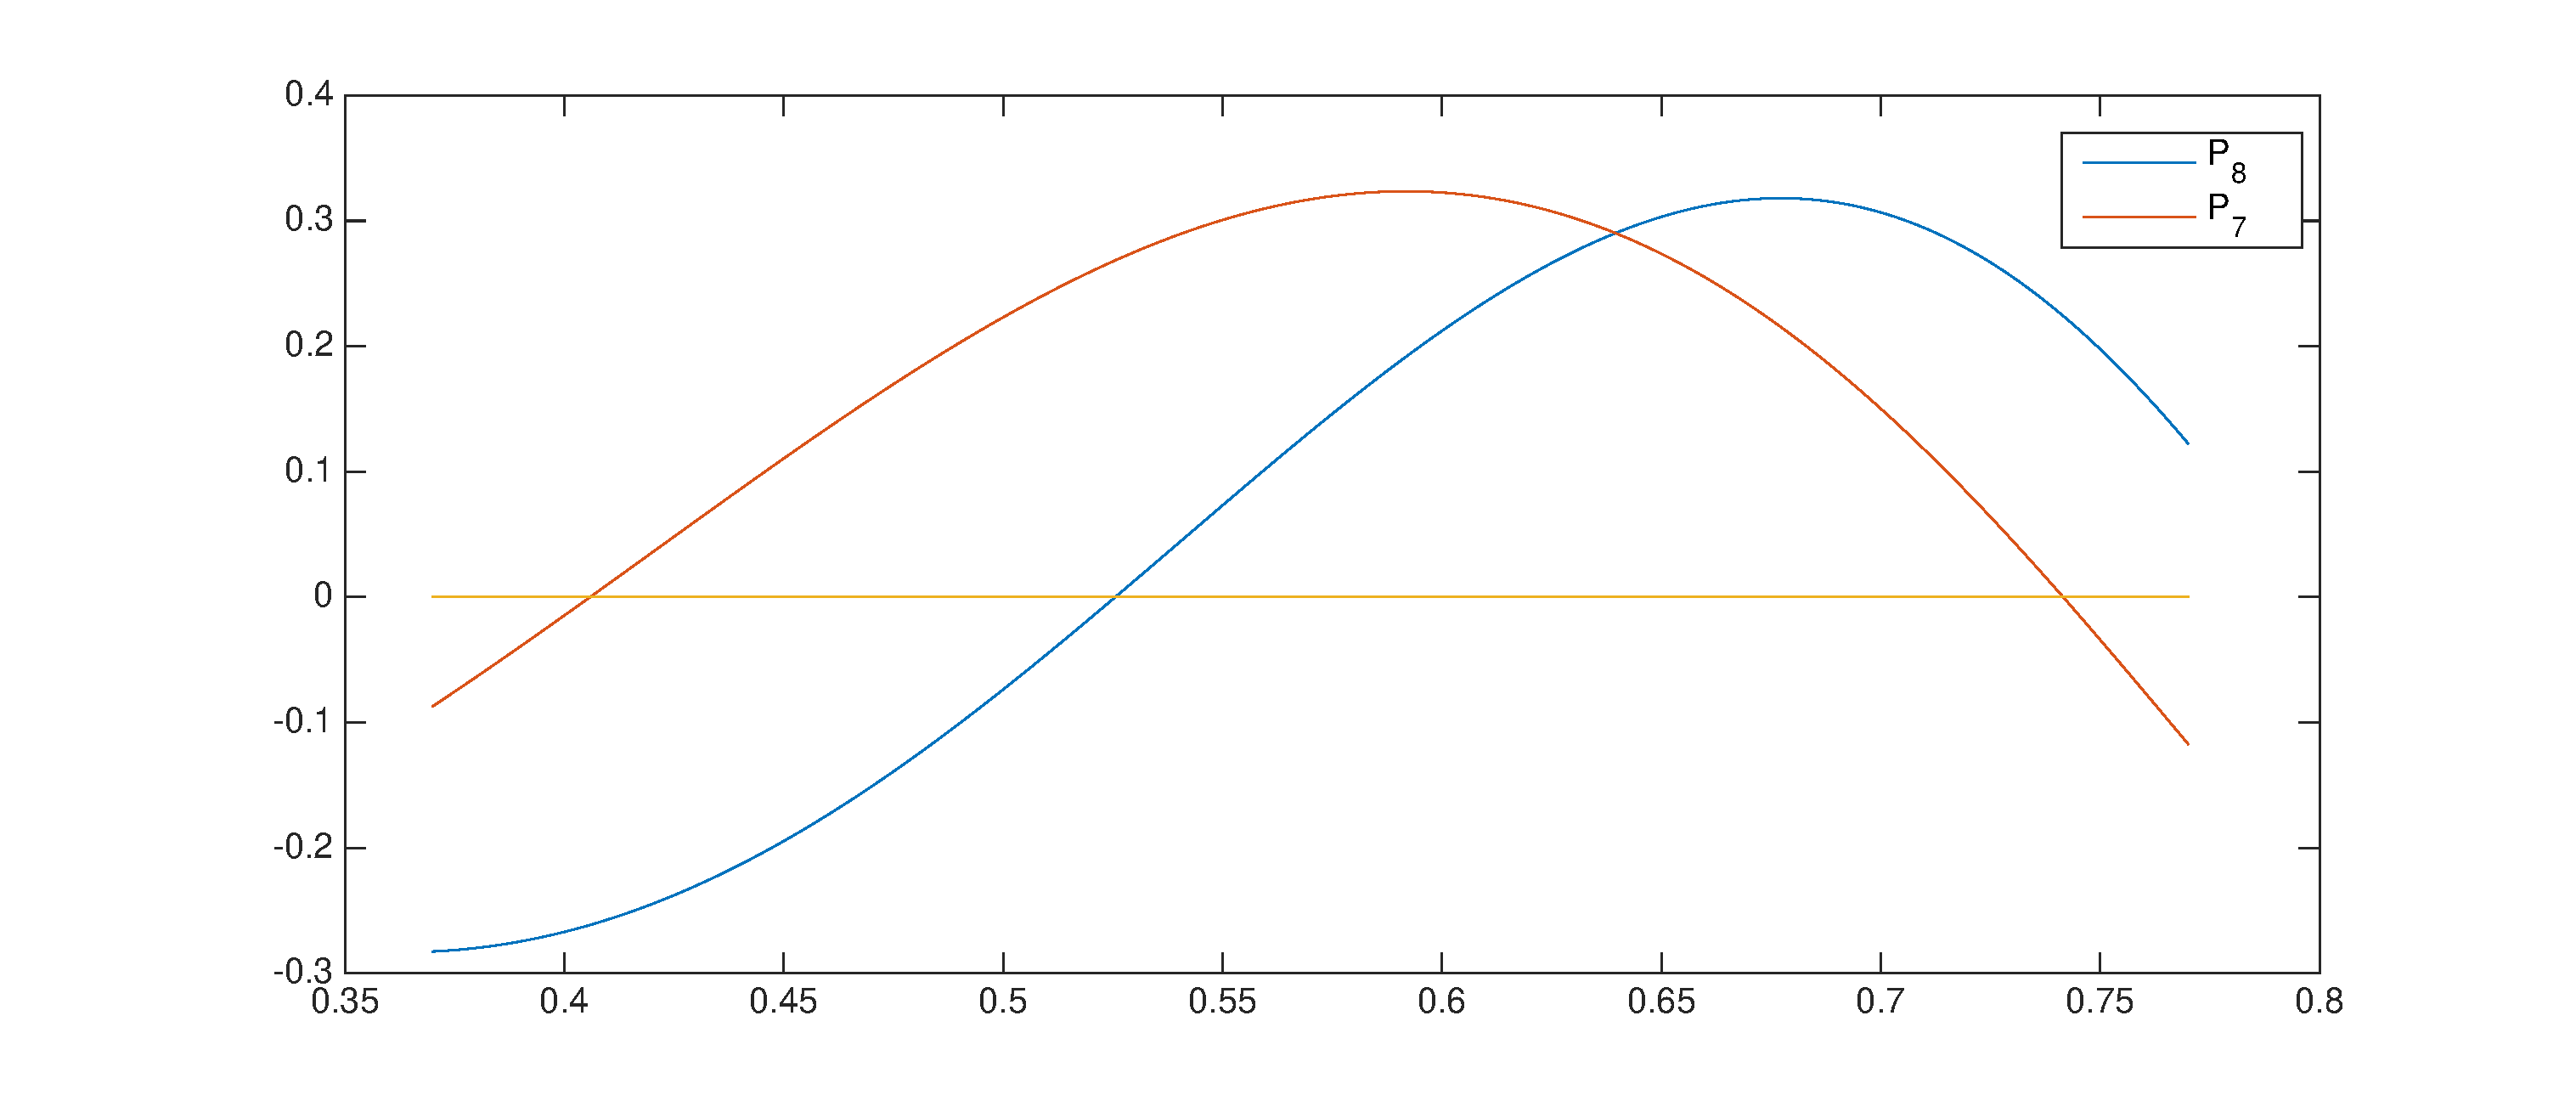
\includegraphics[width=.9\textwidth]{\problems/ch_numericalquadrature/PICTURES/secant.eps}
\caption{$P_7$ and $P_8$ on a part of $[-1,1]$. The secant method fails to find the zeros of $P_8$ (blue curve) when started with the zeros of $P_7$ (red curve).}
\label{fig:secant}
\end{figure}
\end{hint}
\begin{solution}
See file \texttt{legendre.cpp} for the implementation. The zeros of $P_k$, $k=1,\dots,7$ are all correctly computed, but the zero $\xi^8_6\approx 0.525532$ of $P_8$ is not correct. This is due to the fact that in this case the initial guesses for the secant method are not close enough to the zero (remember, only local convergence is guaranteed). Indeed, taking $x^{(0)}$ and $x^{(1)}$ as the two consecutive zeros of $P_7$ in Figure~\ref{fig:secant}, the third iterate $x^{(2)}$ will satisfy $P_8(x^{(1)})P_8(x^{(2)})>0$ and the forth iterate will be very far from the desired zero.
\end{solution}
\end{subproblem}

% SUBPROBLEM 6
\begin{subproblem}[2]
Fix your function \texttt{gaussPts} taking into account the above considerations. You should use the \emph{regula falsi}, that is a variant of the secant method in which, at each step, we choose the old iterate to keep depending on the signs of the function. More precisely, given two approximations $x^{(k)}$, $x^{(k-1)}$ of a zero in which the function $f$ has different signs, compute another approximation $x^{(k+1)}$ as zero of the secant. Use this as the next iterate, but then chose as $x^{(k)}$ the value $z \in \{ x^{(k)} ,x^{(k-1)}\}$ for which $ {\rm sign} f(x^{(k+1)}) \neq {\rm sign} f(z)$. This ensures that $f$ has always a different sign in the last two iterates.
\begin{hint}
The regula falsi variation of the secant method can be easily implemented with a little modification of \lref{mc:secant}:
\begin{lstlisting}
function x = secant_falsi(x0,x1,F,rtol,atol)
fo = F(x0);
for i=1:MAXIT
  fn = F(x1);
  s = fn*(x1-x0)/(fn-fo); % correction
  if (F(x1 - s)*fn < 0)
    x0 = x1;  fo = fn;  end
  x1 = x1 - s;
  if (abs(s) < max(atol,rtol*min(abs([x0;x1]))))
    x = x1; return; end
end  
  \end{lstlisting}
\end{hint}
\begin{solution}
See file \texttt{legendre.cpp}.
\end{solution}
\end{subproblem}

\end{problem}




